% 图 8.12 La2CuO4 中的 CuO2 面：Cu 格点（实心方点，反铁磁交替箭头），O 位于键中点（空心圆）
\documentclass[tikz,border=5pt]{standalone}
\usetikzlibrary{arrows.meta}
\usepackage{amsmath}
\usepackage{bm}
\usepackage{fontspec}
\setmainfont{Times New Roman}
\begin{document}
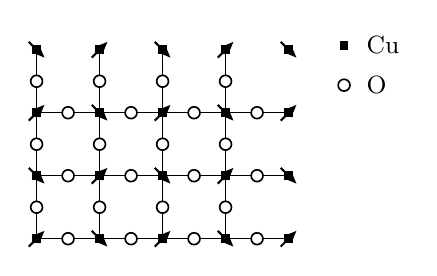
\begin{tikzpicture}[line width=0.8pt,>=Stealth]
  % bond grid
  \foreach \y in {0,0.8,...,2.4}{ \draw[line width=0.5] (0,\y) -- (3.2,\y); }
  \foreach \x in {0,0.8,...,3.2}{ \draw[line width=0.5] (\x,0) -- (\x,2.4); }
  % oxygen at bond midpoints
  \foreach \y in {0,0.8,...,2.4}{
    \foreach \x in {0.4,1.2,...,2.8}{ \draw[fill=white,line width=0.6] (\x,\y) circle (0.075); }}
  \foreach \x in {0,0.8,...,3.2}{
    \foreach \y in {0.4,1.2,...,2.0}{ \draw[fill=white,line width=0.6] (\x,\y) circle (0.075); }}
  % copper sites with alternating AFM arrows
  \foreach \i in {0,...,4}{
    \foreach \j in {0,...,3}{
      \pgfmathsetmacro{\x}{\i*0.8}
      \pgfmathsetmacro{\y}{\j*0.8}
      \pgfmathtruncatemacro{\s}{mod(\i+\j,2)}
      \ifnum\s=0
        \draw[->,line width=0.75,-{Stealth[length=1.6mm,width=1.3mm]}]
          ({\x-0.100},{\y-0.100}) -- ({\x+0.100},{\y+0.100});
      \else
        \draw[->,line width=0.75,-{Stealth[length=1.6mm,width=1.3mm]}]
          ({\x-0.100},{\y+0.100}) -- ({\x+0.100},{\y-0.100});
      \fi
      \fill[black] ({\x-0.055},{\y-0.055}) rectangle ({\x+0.055},{\y+0.055}); }}
  % legend
  \fill[black] (3.85,2.40) rectangle (3.96,2.51);
  \node[right] at (4.06,2.455) {\small Cu};
  \draw[fill=white,line width=0.6] (3.905,1.95) circle (0.075);
  \node[right] at (4.06,1.95) {\small O};
\end{tikzpicture}
\end{document}
